\subsection{Train and validate considering all sensors}
In the previous section, an extensive test of the framework has been performed on a single signal from the dataset (Bearing 3 x). So the warning given by the \gls{mla} was detecting a problem in a specific component of the maintained system. Let's now test a configuration that takes into account all the signals of the dataset, so all eight signals from the four bearings are used for \gls{glo:feature} extraction. This configuration should be able to detect a generic novel behaviour of the system or, better, a situation in which the system is abnormal as a whole (the signals may be normal but the combination of them may be abnormal).  In this case, the configuration file has been set to use all the time-domain and all the frequency-domain \gls{glo:feature}s, and the \gls{mla} has been trained with the same procedure as before, with the first 600 \gls{glo:snap}s of the dataset. 


\begin{figure}
    \centering
    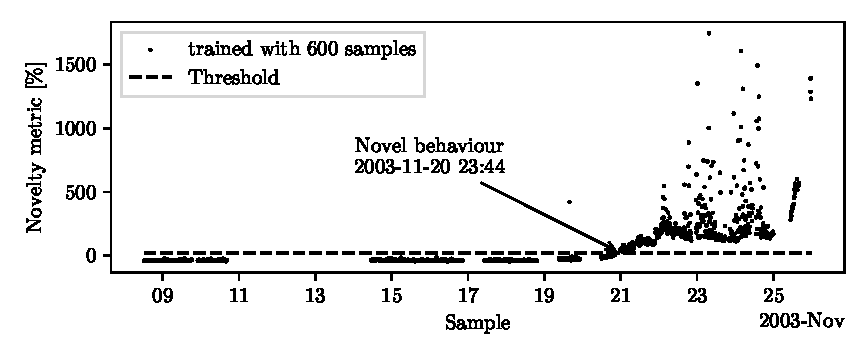
\includegraphics{images/IMS/Novelty_01_500samples_allsensors.pdf}
    \caption{Novelty detection on the \gls{ims} dataset No.1 using all the sensors}
    \label{fig:IMS_n1_allsensors}
\end{figure}

In \autoref{fig:IMS_n1_allsensors}, the evolution of the novelty metric over time is shown. Ignoring an outlier that appeared at the end of 2003-11-19, the \gls{nd} event triggered at 2003-11-20 23:44, 5~days before the end of the data acquisition. After the event, the novelty metric stays consistently over the threshold.

Let's compare now this result to the classic approach of just using the \gls{rms} of the signals. The maximum value of the \gls{rms} among all the bearings is shown in \autoref{fig:IMS_n1_allsensors_RMS}. It is clear that the \gls{ml} approach is much more robust, as there is no threshold that would have both minimised the false positives and triggered a \gls{nd} event sufficiently in advance.

\begin{figure}
    \centering
    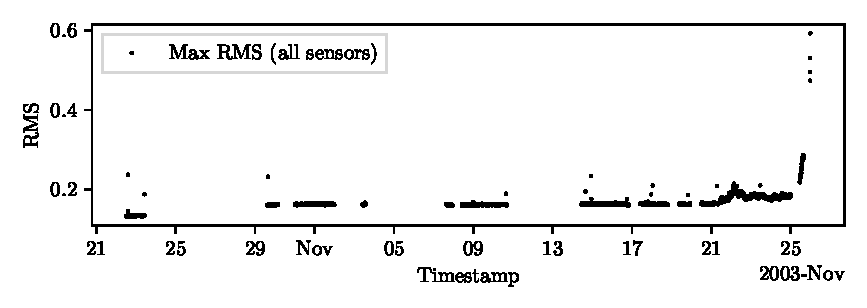
\includegraphics{images/IMS/Novelty_01_RMS_allsensors.pdf}
    \caption{Maximum value of \gls{rms} vibration among all bearings}
    \label{fig:IMS_n1_allsensors_RMS}
\end{figure}

Knowing that the \gls{nd} event is triggered at 2003-11-20 23:44, the \gls{rul} prediction is shown in \autoref{fig:IMS_n1_allsensors_prediction}. The Predictions are made considering the last 250 \gls{glo:snap}s of the dataset, and the \gls{rul} is predicted at different instants after the \gls{nd} event. Most predictions are accurate, except for the one done on 2003-11-23 00:00, which is affected by the temporary local decrease of the novelty metric. In this case, the last \gls{rul} should be retained, as the system is still in a novel state.

\begin{figure}
    \centering
    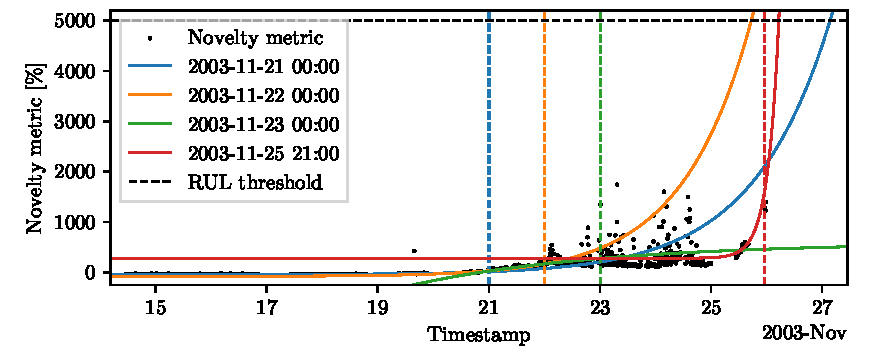
\includegraphics[width=\textwidth]{images/IMS/Novelty_01_500samples_allsensors_predictions.pdf}
    \caption{\gls{rul} prediction at different instants after the \gls{nd} event (dashed lines are the instants of the predictions corresponding to the same-colour solid line prediction)}
    \label{fig:IMS_n1_allsensors_prediction}
\end{figure}